\section{Part A}%
\label{a}


\begin{figure}[H]
	\centering
	\captionsetup{justification=centering}
	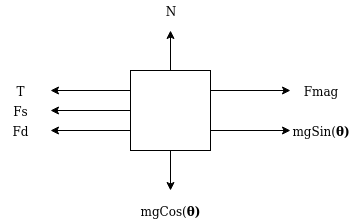
\includegraphics[width=0.8\linewidth]{imgs/FBD.png}
	\caption{Free-body diagram of forces acting upon the ball}%
	\label{fig:14}
\end{figure}

Forces on x-axis : \\
\[
Fmag + mg \sin (\theta ) - T - Fs - Fd = m \ddot x\label{eq:1} \tag{\ding{1}}
\]

$Fs = k(x-d)$\\
$Fd = b\dot x$


Forces on y-axis: \\
$N - mg\cos(\theta) = 0$  - (2)

Moment of inertia, i = $2/5mr^2$

Torque $M = -Tr$          (-Ve as rotating clockwise)

$I\ddot \theta = -Tr \rightarrow  1/2 mr^{\cancel{2}} \ddot\theta = -T\cancel{r}$

$T = -1/2 mr\ddot\theta$ 

By 'Pizza slice theorem', $\ddot x = \ddot \theta r$

Therefore, 
$T = 1/2 m \ddot x$ \\

Finding magnet force, Fmag

$Fmag = C \frac{I^2}{R^2}$    -  (2)

Applying Kirchoffs Voltage Law on loop,\\
$V = IR + \dot I C$

$$\int V dy = IR \int 1\cdot dy + C \int \frac{di}{dy} dy$

$Vy = IRy + LI$

$Vy = I(Ry + L)$

$I = \frac{Vy}{Ry+L}$ -   (3)

Substituting (3) into (2)

$Fmag = \frac{CV^2y^2}{(Ry + L)^2 y^2} = \frac{C}{(Ry+L)^2}V^2$ - (4)

Substituting (4) into (1)

$$\frac{CV^2}{(Ry+L)^2} + mg\sin(\theta) -k(x-d) - b\dot x = \frac{1}{2}m\ddot x $

\textbf{A2}  \\

    $x_{1} = x$
    
   $x_{2} = \dot x_{1} = \dot x$
   
    $\dot x_{2} = \ddot x$
    
    

    \underline{x}=
\left\{\begin{matrix}
\dot x = x_{2}
\\ 
\frac{2CV^2}{(Ry+L)^2m} + 2g\sin(\theta) - \frac{2k}{m}(x_{1}-d) - \frac{2b}{m} x_{2} = \dot x_{2}
\end{matrix}\right.

\textbf{A3}  \\

$\dot x = f(x, V)$, a pair $(x^eq , V^eq)$ is an equilibrium point if $f(x^eq, V^eq) = 0$
\\


at equilibrium, $d = 0$

    $\underline{x^{eq}}=$
\left\{\begin{matrix}
x_{2}^{eq} = 0
\\ 
\frac{2CV^2}{(Ry+L)^2m} + 2g\sin(\theta) - \frac{2k}{m}(x_{1}^{eq}-0) - \frac{2b}{m} x_{2}^{eq} = 0
\end{matrix}\right.
\\
\\
\pagebreak \\
\textbf{A4} \\
\frac{2CV^2}{(Ry+L)^2m} + 2g\sin(\theta) - \frac{2k}{m}(x_{1}^{eq}-d) - \frac{2b}{m} x_{2}^{eq} = 0

$g(V) = V^2$

$g'(V) = 2V$

$g(V^eq) = (V^eq)^2$

$g'(V^eq) = 2V^eq$

By Taylor's Theorem, 

$g(V)\approx g(V^{eq}) + g'(V^{eq})(V - V^{eq})$ \\
$V^2 \approx (V^{eq})^2 + 2V^{eq} (\bar{V})$ \\

Deviation variable, $\bar{V}$ \\

$V^2 \approx (V^{eq}^2 + 2(V^{eq})(\bar{V})$ \\
$V^2 - (V^{eq})^2 \approx 2(V^{eq})(\bar{V})$

$\dot x_{2} - \dot x_{2}^{eq} = \dot x_{2} - 0 = \dot x_{2} = \dot\bar x_{2}$

$\dot x_{2} - \dot x^{eq}^{2}$

 $\dot \bar x_{2} = \frac{2c}{m(Ry + L)^2}2V^{eq}\cdot V - \frac{2k}{m}(x_{1}-x_{1}^{eq}) - \frac{2b}{m} (x_{2}-x_{2}^{eq})$
 
 Using deviation variables, \\
 $\bar x_{1} = (x_{1}-x_{1}^{eq})$ \\
 $\bar x_{2} = (x_{2}-x_{2}^{eq})$  \\
 $\bar V =  2V^{eq}\cdot V$ \\
 
 $ \dot \bar x_{2} =
\begin{bmatrix}
\frac{2c}{m(Ry + L)^2} \end{bmatrix} \bar V- \begin{bmatrix}\frac{2k}{m}\end{bmatrix}\bar x_{1} - \begin{bmatrix}\frac{2b}{m}\end{bmatrix} \bar x_{2}
$ \\

 $ \dot \bar x_{2} = A \bar V - B\bar x_{1} - C\bar x_{2}$
 
\textbf{A5} \\
Finding transfer function,\\
$x_{2} = \dot x_{1} \quad x_{2}^{eq} = 0$ \\
$x_{2} - x_{2}^{eq} = \dot x - 0$ \\
$\bar x_{2} = \dot x_{1}$ \\
$\bar x_{2} = \dot \bar x_{1}$ \\
$\dot \bar x_{2} = A\bar V - B\bar x_{1} - C\dot \bar x_{1}$ \\ 
$S \cdot \bar x_{1} = \bar x_{2} = \dot \bar x_{1}$ \\ 
$S \cdot \bar x_{2} = \dot \bar x_{2}$ \\
$\therefore S\bar x_{2} =  A\bar V - B\bar x_{1} - C(S \cdot \bar x_{1})$ \\
$S \bar x_{2} = S \cdot S \cdot \bar x_{1}$ \\
$S^2 \bar x_{1} = A\bar V - B$ \\
$S^2\bar x_{2} =  A\bar V - B\bar x_{1} - C(S \cdot \bar x_{1})$ \\
$S^2\bar x_{2} + B\bar x_{1} + C(S \cdot \bar x_{1}) =  A\bar V$ \\
$(S^2 + B + CS)\bar x_{1} = A\bar V$ \\
Re-arranging to get transfer function, \\
$\frac{\bar x_{1}}{\bar V} = \frac{A}{S^2 + CS + B}$ \\